\subsection{Overview}
\subsection{Component view}
The following component diagram highlights the main components of the system and their interaction with external entities and services. In the diagram, the components have 
been organized to highlight the logical grouping of the system elements.\\The WebApplication component represents the presentation layer of the system, being the only entry point for the users.
The application and integration logic are represented together due to their tight interaction, while the data layer contains the databases accessed by the respective microservices.
Different colors are used to highlight components that share similar roles in the system.\\ \textcolor{orange}{Orange} components represents the system's microservices. Some complex microservices have been further decomposed into subcomponents, for a more fine grained representation.\\
\textcolor{red}{Yellow} components represents the model of the database accessed by its microservice. The model offers to the microservice an abstraction of the database, allowing it to access the data without knowing the underlying database implementation technology.\\ 
The \textcolor{violet}{violet} has been used to highlight components that cover an important role in the integration between some of the main microservices of the system. Specifically, it has been used for the queues subcomponents, which are used to implement the asynchronous and concurrent communication between specific microservices.
Some microservices have an important role in the integration with external entities as well, but have been depicted with their orange color used for microservices. This aspect will be clarified in the detailed description of the components that follows the diagram.\\
\textcolor{red}{Red} components represent the external services that interact with the system.\\
Finally, the \textcolor{green}{green} color has been used to highlight the databases components that are used to store the data of the system.\\
\begin{figure}[H]
    \centering
    \vspace{-3cm}
    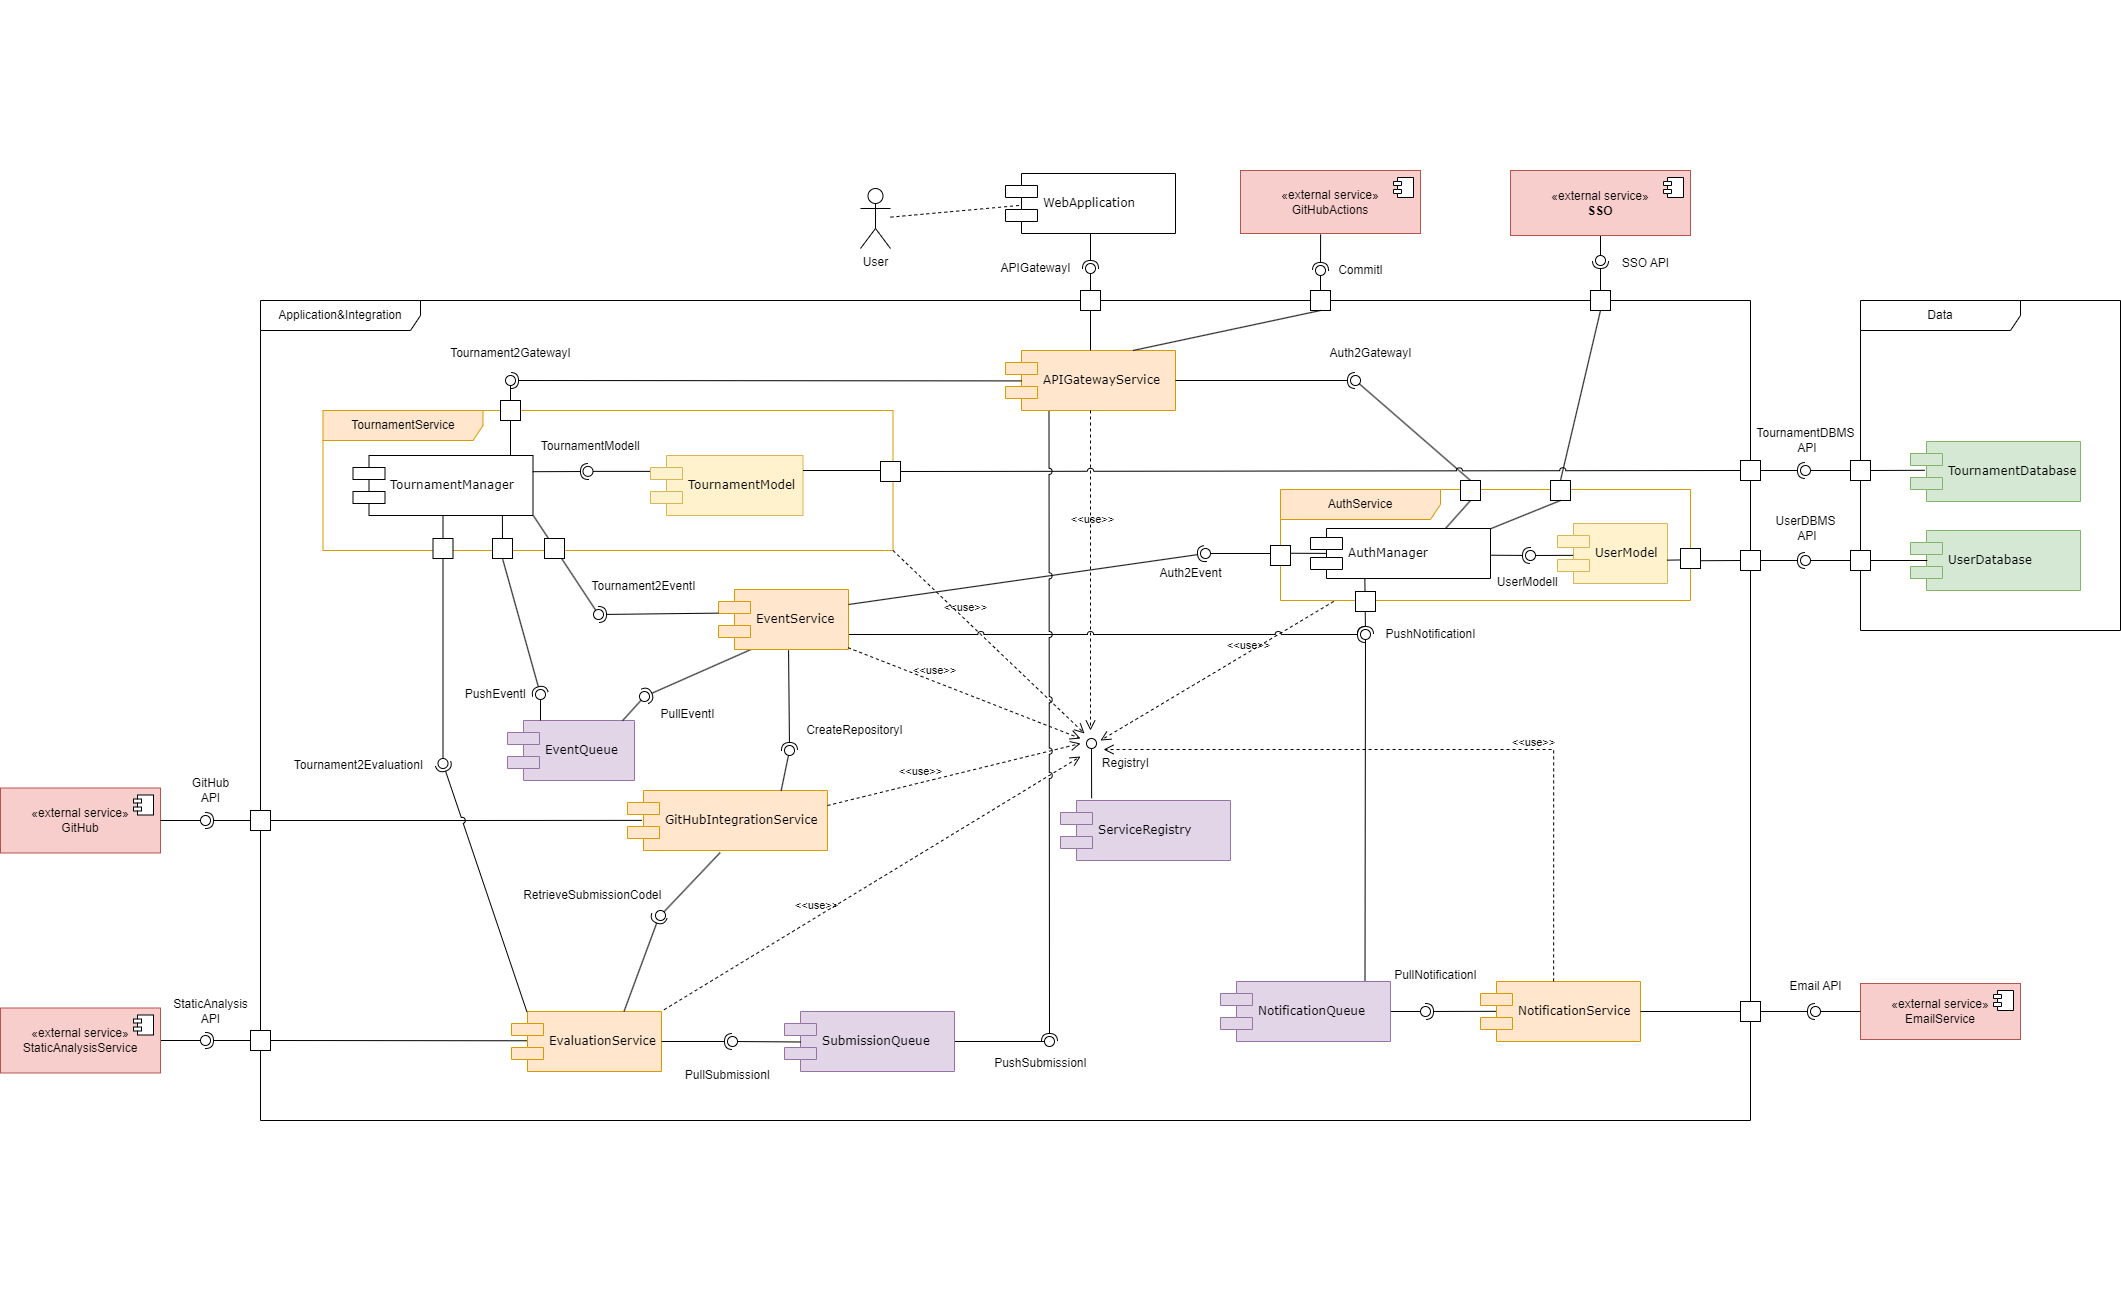
\includegraphics[width=1.6\textwidth,angle=90,origin=c]{Diagrams/component_diagram.png}
    \caption{Component diagram}
\end{figure}


\subsection{Deployment view}
\subsection{Component interfaces}
\subsection{Runtime view}
\subsection{Selected architectural styles and patterns}
\subsection{Other design decisions}